\documentclass[10pt,landscape]{article}

%encoding
\usepackage[T1]{fontenc}
\usepackage[utf8]{inputenc}
\usepackage{lmodern}

%language
\usepackage[english]{babel}

%paper and text body handling
\usepackage{geometry}
\usepackage{setspace}
\usepackage{lettrine}

%graphics
\usepackage{graphicx}
\usepackage[format = plain, labelfont = {bf, it}, textfont = it]{caption}%font settings for captions
\usepackage{xcolor}
\usepackage{pdfpages}
\usepackage{subcaption}
\usepackage{tcolorbox}
\usepackage{multicol}
\usepackage{tikz}
\usetikzlibrary{arrows.meta}
\usetikzlibrary{bending}


%code
%\usepackage{minted}

%math
\usepackage{amsmath}%math
\usepackage{amssymb}%
\usepackage{amsfonts}%
\usepackage{amsthm}%theorems
\usepackage{aligned-overset}
\usepackage{siunitx}
\usepackage{cancel}
\usepackage{braket}
\usepackage{bm}
\usepackage{diffcoeff}
\usepackage{bbold}
% Use the correct ds in diffs
\diffdef{}{
  op-symbol = \mathrm{d},
  op-order-sep = 0 mu
}

%links
\usepackage[colorlinks=true,
            linkcolor=red,
            urlcolor=blue,
            citecolor=gray]{hyperref}


% Specific to this paper
\newcommand{\maj}{\succ}
\newcommand{\majby}{\prec}
%special letters
\newcommand{\R}{\mathbb{R}}
\newcommand{\C}{\mathbb{C}}
\newcommand{\Z}{\mathbb{Z}}
\newcommand{\N}{\mathbb{N}}
\newcommand{\F}{\mathcal{F}}
\newcommand{\PP}{\mathbb{P}}
\newcommand{\EE}{\mathbb{E}}
\newcommand{\idty}{\mathbb{1}}

%functions
\renewcommand{\Re}{\textnormal{Re}}
\renewcommand{\Im}{\textnormal{Im}}
\DeclareMathOperator{\Var}{Var} % Variance
\DeclareMathOperator{\Cov}{Cov} % Covariance
\DeclareMathOperator{\Res}{Res} % Residue
\DeclareMathOperator{\Ker}{Ker} % Kernel
\DeclareMathOperator{\tr}{tr} 	% Trace
\newcommand{\scalprod}[2]{\left\langle#1, #2\right\rangle}

\DeclarePairedDelimiter\abs{\lvert}{\rvert}%
\DeclarePairedDelimiter\norm{\lVert}{\rVert}%

% Swap the definition of \abs* and \norm*, so that \abs
% and \norm resizes the size of the brackets, and the
% starred versions do not.
\makeatletter
\let\oldabs\abs
\def\abs{\@ifstar{\oldabs}{\oldabs*}}
%
\let\oldnorm\norm
\def\norm{\@ifstar{\oldnorm}{\oldnorm*}}
\makeatother

%symbols
% for := as
\newcommand*{\defeq}{%
    \mathrel{%
        \vcenter{%
            \baselineskip0.5ex \lineskiplimit0pt \hbox{\scriptsize.}\hbox{\scriptsize.}%
        }%
    }%
    =%
}


%settings

%spacing
\renewcommand{\arraystretch}{1.2}
\setlength{\arraycolsep}{3pt}

%units
\sisetup{
   output-decimal-marker = {,},
   exponent-product = \ensuremath{\cdot}
}

%text
\makeatletter
   \newlength{\textSize}
   \setlength{\textSize}{\f@size pt}
\makeatother
\setlength{\parindent}{0pt}             % No indentation on new paragraph
%\setstretch{1.15}


%paper and text body
\geometry{
	top=0.5cm,
	bottom=0.5cm,
	left=0.5cm,
	right=0.5cm,
   a4paper,
   centering,
}


%lettrine settings
\setcounter{DefaultLines}{3}


\renewcommand{\vec}{\bm}

\newcommand{\topiccolor}{green}
\renewcommand{\section}[2]{%
	\renewcommand{\topiccolor}{#2}
	\begin{tcolorbox}[boxsep=0.5mm, left=1mm, right=1mm, top=0mm, bottom=0mm,
		colback=#2!30, colframe=#2, arc is angular]%
		\centering \textbf{#1}%
	\end{tcolorbox}%
}
\newcommand{\cbf}[1]{\textcolor{\topiccolor!80!black}{\textbf{#1}}}

\begin{document}

\begin{multicols*}{3}
\begin{tcolorbox}[colframe=black, colback=white]
\centering \large Plasma Physics with Applications\\
\small David Hambr\ae{}us \& Ida Ekmark
\end{tcolorbox}

\section{What is a plasma}{magenta}
A plasma is defined via the \cbf{ionization degree} $\alpha$ defined as the
fraction of ionized particles. At $\alpha > 0.01$ we say it is 
\cbf{fully ionized}, while for smaller $\alpha$:s its 
\cbf{weakly / partially ionized}.

\section{Single particles in EM-field}{blue}

The most fundamental equation of motion for a charged particle in an EM-field is
the \cbf{Lorentz Force Equation:}
\[
	m \diff{\vec v}{t} = q(\vec E + \vec v \times \vec B)
\]
A constant, nonzero E-field with no B-field gives constant acceleration along
$\vec E$. A constant, nonzero B-field with no E-field gives rise to helical
motion with \cbf{cyclotron frequency} $\omega_c = \abs{q} B / m$ and
\cbf{Larmor radius} $r_L = v_\perp / \omega_c$.
A constant, nonzero B-field with a constant force $\vec F$ gives a constant
acceleration from the component of $\vec F$ along the B-field, while the
component perpendicular to $\vec B$ gives rise to a constant \cbf{drift velocity}
\[
	\vec v_D = \frac1q \frac{\vec F_\perp \times \vec B}{B^2}
\]
An \emph{inhomogeneous} B-field gives rise to the so called \cbf{grad B drift}.
The motion parallel to the B-field lines is governed by
\[
	m \diff{\vec v_\parallel}{t} = - \mu \nabla_\parallel B,
\]
and for the motion perpendicular we get a drift velocity
\[
	\vec v_D = \frac\mu q \frac{\vec B \times \nabla B}{B^2}
\]
in addition to the Larmor rotation, just like before.
\begin{center}
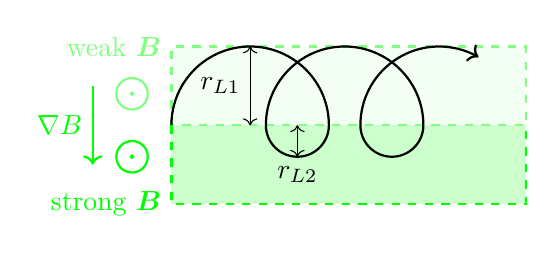
\begin{tikzpicture}[thick]
	\draw[draw=\topiccolor, dashed, fill=\topiccolor!20] (0,0) rectangle (4.5,-1);
	\draw[color=\topiccolor] (-0.5,-0.4) circle[radius=0.2]
		circle[radius=0.014];
	\node at (0,-1) [anchor=east, color=\topiccolor] 
		{strong $\vec B$};

	\draw[draw=\topiccolor!50, dashed, fill=\topiccolor!5] (0,0) rectangle (4.5,1);
	\draw[color=\topiccolor!50] (-0.5,0.4) circle[radius=0.2]
		circle[radius=0.014];
	\node at (0,1) [anchor=east, color=\topiccolor!50] 
		{weak $\vec B$};

	\draw[->, color=\topiccolor] (-1, 0.5) -- node[anchor=east]{$\nabla B$}
		(-1, -0.5);

	\draw[->] (0,0) 
		arc[start angle=180, end angle=0, radius=1]
		arc[start angle=0, end angle=-180, radius=0.4]
		arc[start angle=180, end angle=0, radius=1]
		arc[start angle=0, end angle=-180, radius=0.4]
		arc[start angle=180, end angle=60, radius=1];
	\draw[thin, <->] (1,0) -- node[anchor=east]{$r_{L1}$} (1,1);
	\draw[thin, <->] (1.6,0) -- (1.6,-0.4) node[anchor=north]{$r_{L2}$};

\end{tikzpicture}
\end{center}
TODO: \cbf{Curved fields}

\section{The Vlaslov and Boltzmann equations}{green}

Firstly we define a \cbf{distribution function}, $f(\vec r, \vec v, t)$.
This gives the expected number of particles occupying the volume in
phase space $\dl \vec r \dl \vec v$ around the point $(\vec r, \vec v)$
at time $t$.
To understand how this $f$ evolves argue that the rate of change of the
number of particles inside some volume in phase space $\Omega$ must
be the flux of particles through the walls.
\[
	\diffp*{\int_\Omega f \dl \vec r \dl \vec v}{t}
	= -\int_{\partial_r \Omega} f \vec v \cdot \hat n_r \dl S_r
	-\int_{\partial_v \Omega} f \vec a \cdot \hat n_v \dl S_v.
\]
$\partial_r \Omega$ means the boundry of $\Omega$ in r-space.
Plopping the $\diffp{}{t}$ into the integral and using Gauss' theorem to
make the surface integral a volume integral we obtain
\[
	\dl \vec r \dl \vec v 
	\left[\diffp f t + \diffp{}{\vec r} \cdot \vec v f
	+ \diffp{}{\vec v} \cdot \vec a f
	\right]
	=0,
\]
which has to be true for all volumes, meaning that the integrand has
to be 0 everywhere.
Further noting that $\diffp{}{r} \cdot \vec v = 0$ and plugging in the
Lorentz force for the acceleration we get the \cbf{Vlaslov equation}
\[
	\diffp f t + \vec v \cdot \diffp{f}{\vec r} 
	+ \frac q m(\vec E + \vec v \times \vec B) \cdot \diffp{f}{\vec v} = 0.
\]
The LHS is really the change of $f$ along a particle trajectory (if you let
$\vec r(t)$ and $\vec v(t)$ be the particle position and velocity at time t),
so you can let $f$ be the sum of a bunch of delta functions and reduce this to
the particle description of the plasma.
But this would not be very useful, instead we let $f$ be some smooth
distribution.
This is okay if the collective effect of far away particles are more important
than the effects of collisions.
If we want to include the effects of collisions, we add a mysterious term called
the collision operator to obtain the \cbf{Boltzmann equation}
\[
	\diffp f t + \vec v \cdot \diffp{f}{\vec r} 
	+ \frac q m(\vec E + \vec v \times \vec B) \cdot \diffp{f}{\vec v} 
	= \left(\diffp f t\right)_c.
\]

For plasmas in equilibrium, $\diffp f t = 0$ since they are by definition
stationary in time. This also means that the net flux out of any volume
in phase space must be 0. TODO why does this mean that the collision operator
must be 0?

\section{The two fluid model}{olive}

In this model, we try to simplify the equations above by not caring about the
true $f$, but rather we treat the plasma as a fluid and only care about some of
its moments.
A moment $\expval{\psi}$ is defined as the velocity average
of the function $\psi$:
\[
	\expval{\psi} = \frac1n \int \psi f \dl \vec v,
\]
where $n$ is the density of particles $n(\vec r) = \int f \dl \vec v$.
Using the Boltzmann equation we can derive the \cbf{general moment equation}
\[
	\begin{split}
		\diffp*{(n \expval \psi)}{t} + \nabla \cdot (n \expval{\vec v \psi})
		- \frac{nq}{m} \expval{(\vec E + \vec v \times \vec B) \cdot
		\diffp{\psi}{\vec v}}\\
		= \diffp*{(n\expval{\psi})_c}{t}
	\end{split}
\]
This gives a way of solving the time evolution of these microscopic properties
instead of dealing with $f$ directly.
However, the problem as you can see in the second term is that the equation for
the order $k$ moment contains the order $k+1$ moment.

As an easy example, consider the equation for the zero order moment ($\psi =
1$).
It becomes
\[
	\diff{n_\alpha}{t} + \nabla \cdot (n_\alpha \vec u_\alpha) = 0.
\]
$\vec u_\alpha$ is here the average velocity of the particles of species
$\alpha$ at $\vec r$.
The is basically the continuity equation.
As you can see, it does depend on the average velocity,
and the equation for the average velocity depends on the pressure tensor
(a second order moment) and so on.
Somewhere we have to cut it.


\end{multicols*}

\end{document}

